%========================================================
\section{Estimation of Model Parameters}
\label{sec:estimation}
%========================================================
This section describes the estimation framework used in CICADAS. The goal is to construct a fully
specified generative model for disease burden, treatment effects, and mortality that can serve as the
kernel of the parametric g-formula. Full derivations, filter recursions, and implementation details
are given in the Supplementary Material; what follows is the logic of the procedure.

\paragraph{Plain-English preview.} The estimation problem has three pieces. \emph{First}, we use
untreated patients to learn how epileptiform activity evolves on its own (the disease-dynamics
parameters). Because untreated patients receive no drug, the observed severity trajectory is a direct
read-off of the underlying disease process. \emph{Second}, we use patients whose dose changes during
the ICU stay to learn how the drug affects severity (the PK/PD parameters). These patients provide
enough variation in exposure to separate the drug's effect from the background disease dynamics;
patients on constant closed-loop control do not. \emph{Third}, we use the full cohort to learn how
cumulative disease burden and cumulative treatment burden combine into a death hazard (the outcome
parameters). Once these three components are fitted, we simulate counterfactual trials under
alternative dosing policies by forward Monte Carlo from the fitted generative model and compare the
resulting survival curves---this is the g-formula in operation.

%--------------------------------------------------------
\subsection{Overview}
%--------------------------------------------------------
CICADAS proceeds in two phases. \textbf{Phase 1 (model estimation)} constructs the generative model by
estimating its components from observed data, in three stages: disease natural history, PK/PD
parameters, and the mortality hazard. \textbf{Phase 2 (trial emulation)} applies the parametric
g-formula to the fitted model, simulating counterfactual outcomes for the whole cohort under
alternative dynamic treatment strategies and producing counterfactual survival curves and policy
contrasts. Figure~\ref{fig:pipeline} shows the full workflow.

When CICADAS is applied to real ICU data, Phase~2 is the causal effect estimator. In this paper, where
all data are simulated, we additionally generate synthetic datasets from a known data-generating
process and reapply the same trial emulation to assess whether it recovers the causal effects that are
true by construction (Section~\ref{ssec:validation-framework}).

\begin{figure}[htbp]
\centering
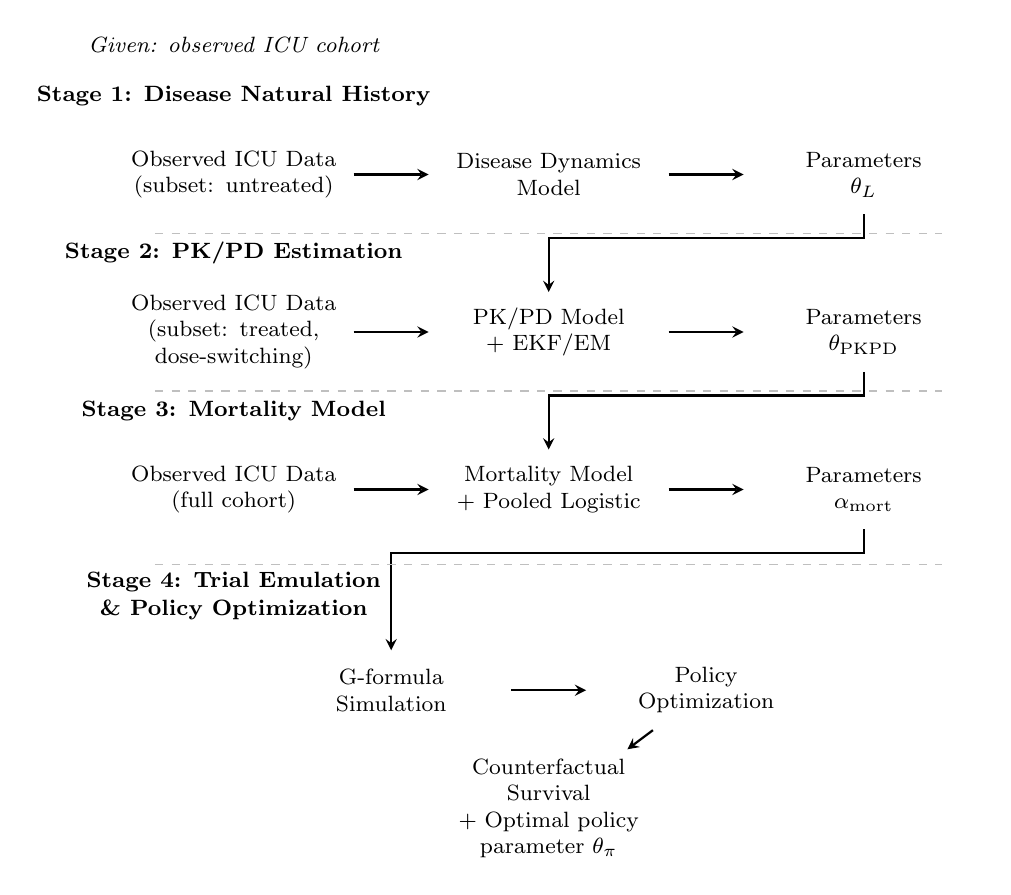
\begin{tikzpicture}[
    node distance=1.5cm and 3cm,
    component/.style={text width=2.8cm, text centered, minimum height=1cm, font=\footnotesize},
    arrow/.style={->, >=stealth, thick, black},
    stage/.style={font=\bfseries\footnotesize},
    note/.style={font=\footnotesize\itshape, text centered}
]

% Starting point (centered over Stage 1 left node)
\node[note] at (0,8.15) {Given: observed ICU cohort};

% Stage titles
\node[stage] at (0,7.5) {Stage 1: Disease Natural History};
\node[stage] at (0,5.5) {Stage 2: PK/PD Estimation};
\node[stage] at (0,3.5) {Stage 3: Mortality Model};
\node[stage] at (0,1.15) {\shortstack{Stage 4: Trial Emulation\\\& Policy Optimization}};


% Stage 1
\node[component] (raw_data1)     at (0,6.5) {Observed ICU Data\\(subset: untreated)};
\node[component] (disease_model) at (4,6.5) {Disease Dynamics\\Model};
\node[component] (disease_params)at (8,6.5) {Parameters\\$\theta_L$};

% Stage 2
\node[component] (raw_data2)     at (0,4.5) {Observed ICU Data\\(subset: treated, dose-switching)};
\node[component] (pkpd_model)    at (4,4.5) {PK/PD Model\\+ EKF/EM};
\node[component] (pkpd_params)   at (8,4.5) {Parameters\\$\theta_{\mathrm{PKPD}}$};

% Stage 3
\node[component] (raw_data3)     at (0,2.5) {Observed ICU Data\\(full cohort)};
\node[component] (mortality_model)at (4,2.5) {Mortality Model\\+ Pooled Logistic};
\node[component] (mortality_params)at (8,2.5) {Parameters\\$\alpha_{\mathrm{mort}}$};

% Stage 4 (moved DOWN slightly for breathing room)
\node[component] (gformula)      at (2,-0.05) {G-formula\\Simulation};
\node[component] (optimization)  at (6,-0.05) {Policy\\Optimization};
\node[component] (survival_curves)at (4,-1.55) {Counterfactual Survival\\+ Optimal policy\\parameter $\theta_{\pi}$};

% Horizontal arrows within stages
\draw[arrow] (raw_data1) -- (disease_model);
\draw[arrow] (disease_model) -- (disease_params);

\draw[arrow] (raw_data2) -- (pkpd_model);
\draw[arrow] (pkpd_model) -- (pkpd_params);

\draw[arrow] (raw_data3) -- (mortality_model);
\draw[arrow] (mortality_model) -- (mortality_params);

\draw[arrow] (gformula) -- (optimization);

% Right-angle arrows between stages (shorter drop to reduce clutter near dashed lines)
\draw[arrow] (disease_params.south) -- +(0,-0.30) -| (pkpd_model.north);
\draw[arrow] (pkpd_params.south) -- +(0,-0.30) -| (mortality_model.north);
\draw[arrow] (mortality_params.south) -- +(0,-0.30) -| (gformula.north);

% Final output arrow
\draw[arrow] (optimization) -- (survival_curves);

% Stage separation lines (nudged to avoid Stage 4 title/arrow crowding)
\draw[gray!50, dashed] (-1,5.75) -- (9,5.75);
\draw[gray!50, dashed] (-1,3.75) -- (9,3.75);
\draw[gray!50, dashed] (-1,1.55) -- (9,1.55);

\end{tikzpicture}
\caption{CICADAS workflow applied to observed ICU data. Stage~1 fits the disease natural-history model using untreated patients, Stage~2 fits PK/PD parameters using treated patients with dose switching, and Stage~3 fits the mortality model using the full cohort, yielding $\theta_L$, $\theta_{\mathrm{PKPD}}$, and $\alpha_{\mathrm{mort}}$. Stage~4 uses these fitted components within the parametric g-formula to emulate counterfactual trials under candidate dynamic treatment policies and to optimize a policy parameter $\theta_{\pi}$.}
\label{fig:pipeline}
\end{figure}

\subsection{Data Structure}
Estimation operates on person-time (long) format: one row per patient per time interval, recording
severity $L_t$, treatment intensity $A_t$, censoring and death indicators, and baseline covariates.
An example is given in Supplementary Table~S2.

\subsection{Step 1: Disease Natural History}
The natural-history parameters $\theta_L$ govern how epileptiform-activity burden would evolve absent
treatment. They are estimated from untreated patients, for whom $L_t = L_{0,t}$ by definition, so that
the observed trajectory identifies the underlying process directly without needing to disentangle a
drug effect. We fit the growth, peak, decay, and volatility parameters of the stochastic
disease-dynamics model of Section~\ref{sec:disease_dynamics} by maximum likelihood over the observed
trajectories. Using untreated patients for this step is what makes the subsequent PK/PD step
identifiable: with the background process pinned down, the residual suppression observed in treated
patients is attributable to drug exposure.

\subsection{Step 2: PK/PD Parameter Estimation}
The PK/PD parameters map treatment intensity to suppression of disease burden. Drug concentration is
unobserved, so the model is a nonlinear state-space system: a latent one-compartment concentration
driven by the observed infusion rate, mapped through a Hill function to multiplicative suppression of
the natural history, with patient-specific potency $C_{50}$ and steepness $\gamma$ modeled as
mixed effects on age and SOFA score.

\paragraph{Why dose-switching observational data are required.}
Identification of $(C_{50},\gamma)$ requires variation in exposure within a patient. A patient held at
a stable dose under effective closed-loop control provides almost no information about the shape of
the dose--response curve, because the observed severity is nearly constant and the concentration
occupies a narrow range. Patients whose dose changes during the stay---because of sedation
interruptions, escalation, or weaning---sweep out a range of concentrations and therefore identify the
curve. This is a substantive design requirement, not a technical convenience: it means the framework
depends on precisely the practice variation described in Section~\ref{sec:clinical-problem}, and a
uniformly protocolized cohort would be uninformative for this step.

\subsubsection*{Estimation procedure}
We fit the state-space model by expectation--maximization, using an extended Kalman filter with a
Rauch--Tung--Striebel smoother for the E-step and closed-form updates for the M-step. The full
recursions, the four alternative estimation strategies we compared (joint estimation, oracle $k_e$,
raw two-stage, and two-stage with bias correction), the design diagnostics used to screen patients for
inclusion, uncertainty quantification, and implementation details are given in Supplementary
Section~S3.

The practically important result, reported in Section~\ref{sec:pkpd-results}, is that the two-stage
estimator with bias correction approaches oracle accuracy without requiring the elimination constant
$k_e$ to be known in advance, whereas joint estimation over all parameters simultaneously is unstable
in the presence of parameter interactions and local optima.

\subsection{Step 3: Mortality Model}
The outcome model is a discrete-time hazard fitted by pooled logistic regression on the full cohort,
in which the log-odds of death in each interval depend on cumulative disease burden, cumulative drug
exposure, elapsed time, and baseline severity, with the disease and drug terms scaled by SOFA score and
age respectively. Pooled logistic regression is used because it approximates the discrete-time hazard
directly and extends naturally to the time-varying covariates that the g-formula must simulate forward.
The fitted hazard, together with the disease and PK/PD components, completes the generative model
required by the g-formula.

\subsection{Design Diagnostics}\label{sec:design_diagnostics}
Before any causal estimate is produced, we recommend reporting a set of design diagnostics that
establish whether the data can support the intended policy comparison: the distribution of dose
conditional on severity, the proportion of person-time spent in a concentration range that identifies
the dose--response curve, the observed range of achieved severity relative to the policy thresholds
being evaluated, and the fraction of person-time censored together with the covariates predicting
censoring. The full set is given in Supplementary Table~S3, and Section~\ref{sec:conditions} states
how each maps onto a precondition for applying the framework to real data.

\subsection{Validating the G-Formula Estimator in Simulation}\label{ssec:validation-framework}
Because all data in this paper are simulated, the causal effect of each policy is known by
construction, which allows a direct test of whether the estimator recovers it. We generate two
parallel cohorts from the same disease and PK/PD models, differing only in the treatment-assignment
mechanism: a randomized cohort, in which assignment is independent of patient characteristics and no
censoring occurs, and an observational cohort, in which sicker patients are preferentially treated and
censoring is informative. The randomized cohort supplies the ground truth, obtained directly as the
difference in survival proportions with no modeling. The estimator is then applied to the
observational cohort alone and its output compared with that ground truth.

Performance is assessed on three criteria: bias of the estimated policy contrast against the ground
truth at 168 hours; coverage of bootstrap confidence intervals; and agreement between the estimated
and true counterfactual survival curves over the whole follow-up rather than at the endpoint alone. We
report the same comparison for naive Kaplan--Meier, stabilized IPTW, and a marginal structural model,
so that the g-formula's performance can be read against alternatives applied to identical data.

\subsection{Sensitivity analyses and benchmarking}\label{sec:sensitivity}

To evaluate the robustness of the CICADAS g-formula to violations of its identification
assumptions and to compare it against alternative causal-inference estimators, we ran four
additional experiments on the simulated observational cohort. Code for all four is provided
in the \texttt{sensitivity/} and \texttt{benchmarks/} subdirectories of the public
repository.

\paragraph{Unmeasured confounding (NUC injection).}
We modified the data-generating process to include a binary confounder
\(U \sim \mathrm{Bernoulli}(0.5)\) that is observed by the clinician but hidden from the
estimator: it shifts the treatment-assignment logit by \(\delta_A\) and the mortality
hazard logit by \(\delta_Y\). For each combination on a \(5 \times 5\) grid of
\((\delta_A, \delta_Y) \in \{0, 0.5, 1.0, 1.5, 2.0\}^2\), we generated 3 cohorts of
\(N = 1500\) patients, ran the full CICADAS g-formula pipeline without access to \(U\),
and recorded the resulting bias in the recovered ATE relative to the oracle RCT ATE that
also experiences \(U\). We additionally computed the Ding--VanderWeele E-value~\cite{vanderweele2017evalue} for the
honest ATE (\(\delta_A = \delta_Y = 0\)) and identified the smallest \(\delta_Y\) at
\(\delta_A = 0\) at which the g-formula ATE changes sign.

\paragraph{Measurement error on the EEG-severity proxy.}
We added independent Gaussian noise with standard deviation \(\sigma \in
\{0, 0.01, 0.025, 0.05, 0.1, 0.2\}\) to each observed value of \(L_t\), clipped at zero,
and re-ran the g-formula pipeline on the perturbed data.

\paragraph{Alternative censoring mechanisms.}
We replaced the baseline treatment-dependent informative censoring with three alternatives:
(i) missing completely at random (flat low rate, independent of covariates);
(ii) strongly outcome-dependent censoring (amplified coefficients on cumulative disease
and treatment burden); and (iii) no censoring at all. We compared recovered ATEs across
regimes.

\paragraph{Benchmarking against alternative estimators.}
We compared the CICADAS g-formula against two alternative causal-inference estimators:
(a) stabilized inverse probability of treatment weighting (IPTW)~\cite{robins2000marginal,cole2008constructing} using a pooled logistic
propensity model on the baseline covariates (age, SOFA, early-phase disease severity);
(b) a marginal structural model (MSM)~\cite{robins2000marginal,hernan2000marginal} fit as a weighted pooled logistic regression for
the discrete-time mortality hazard on time and treatment, using the IPTW weights.
We also report a naive Kaplan--Meier estimate from the same observational data as a
reference for the magnitude of confounding. Targeted minimum-loss estimation (TMLE)~\cite{vanderlaan2006tmle,vanderlaan2011targeted} is
not included here as a direct comparator because established implementations
(\texttt{ltmle}, \texttt{survtmle})~\cite{lendle2017ltmle,benkeser2017survtmle} are in R and including them would introduce a
non-trivial cross-language dependency; we discuss this in Section~7 as a direction for
follow-up work. 95\% confidence intervals for IPTW, MSM, and the naive KM estimator come
from 200-replicate nonparametric subject-level bootstrap; the g-formula CIs use the
1000-replicate bootstrap described earlier in this section.
